\documentclass[a4paper]{article}
\usepackage[hmargin=1in, vmargin=1in]{geometry}
\usepackage{makeidx}
\usepackage{fancyhdr}
\pagestyle{fancy}
\usepackage[pdftex]{graphicx}
\usepackage{amsmath}
\usepackage{listings}
\makeindex
\begin{document}
\begin{center}
\title{Three dimensional coordinates into two dimensional coordinates transformation}\\
\author{Edward Gerhold}
\city{Berlin, Germany}
\date{\today}
\maketitle

Version 0.2.6 (the very much a draft paper)\\
\textbf{Remark} Has to be ordered, corrected, mathematically upgraded and to get more pictures.

This is an active working draft. Which is now totally out of it´s shape this version.

}\\

\end{center}


\tableofcontents\\

\section{Introduction}

On a piece of paper you see three coordinate axes pointing into three
directions in space. In reality these vectors are two dimensional. Because
they point into three directions on the paper, and not into the real space.\\

\begin{figure}[ht]
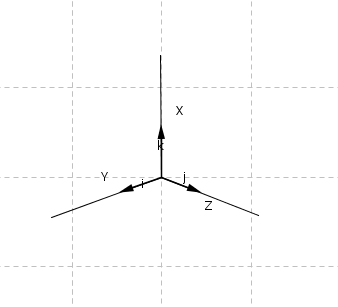
\includegraphics[scale=2]{ijksystem.png}\\
\caption{Picture of a 3-D coordinate system with ijk-vectors on the axes pointing
into three directions. See \cite{Corral1} for introduction.}
\end{figure}

In this document we will design a basis for the coordinate transformation. A
basis is multiplied with the value of the coordinate to move to the correct new point.\\
In the case of cosines and sines, we move left and right and up and down, to 
tell you directly, what happens, when we multiply the coordinates with the matrix.\\

\textbf{What we will do in the document}

\begin{enumerate}
\item Choose angles for our coordinate axes around the unit circle to lay out three axes.
\item Write down the basis vectors for each coordinate axis
\item Assemble a matrix with the vector basis for a point by point transformation.
\item Read the example source code for a computer function, which is exactly two lines long. One for the new $x$ and one for the new $y$.
\item Derive the generic case of transforming coordinate systems down to the plane.
\end{enumerate}

\section{Definitions}

\subsection{Definition of the angles for the coordinate axes}

 Let $\varphi_n$ be the set of axis angles, one for each axis. The angles start
at the same place, at the number zero. You have to arrange the $x$, $y$, and
$z$ axes like on a piece of paper around the unit circle by giving them the
appropriate angles. All three angles start at the default at zero at the horizontal axis of the plane.

\begin{displaymath}
\varphi_n := \{\varphi_x, \varphi_y, \varphi_z\}
\end{displaymath}

\begin{example}
\textbf{Example}
The function rad converts degrees to radians, it´s useful for computer functions taking radians.
\begin{displaymath}
\text{rad}(\phi) := \frac{\pi}{180} \times \phi, \phi \in \mathbb{R}
\end{displaymath}
Here is an example of three angles. The three axes have an angle of 120 degrees between each.
\begin{displaymath}
\varphi_x = \text{rad(210)},
\varphi_y = \text{rad(330)},
\varphi_z = \text{rad(90)} 
\end{displaymath}
\begin{displaymath}
\varphi_x &= \frac{\pi}{180} \times 210 &= \frac{7\pi}{6},  
\varphi_y &= \frac{\pi}{180} \times 330 &= \frac{11\pi}{6}, 
\varphi_z &= \frac{\pi}{180} \times 90 &= \frac{\pi}{2} 
\end{displaymath}
\end{example}

Calculating the three values is fun. More fun with angles could be had with \cite{Corral2}. What the values are good for? The angles have to be passed to the cosine and sine functions, when we setup the basis vectors around a circle.


\subsection{Definition of the three 2-D basis vectors}


Let $e_n$ be the set of three two dimensional basis vectors, namely 
$\vec{e}_x$, $\vec{e}_y$ and $\vec{e}_z$. Other names are $\vec{i}$, $\vec{j}$ or $\vec{k}$ for example, like on the
picture of the coordinate system mentioned. The three vectors point into the three directions
of the three axes. On a piece of paper they are two dimensional, becausee they point into three
directions on the paper. The space being shown is what our brain completes, seeing three correct
axes. The three basis vectors represent exactly one unit into the direction of each axis. This
unit can be manipulated by multiplying the vector components inside $e_n$ with a factor $r_n$.

\begin{displaymath}
e_n := \{\vec{e}_x, \vec{e}_y, \vec{e}_z\}\\
\end{displaymath} 

\begin{figure}[ht]
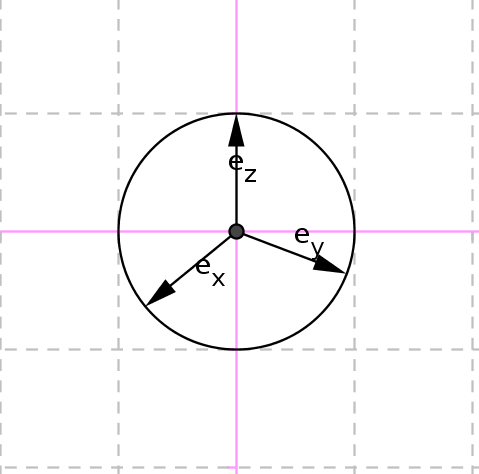
\includegraphics[scale=1]{unitvectors.png}
\caption{The three basis vectors point into the positive directions of the desired coordinate axis. They are arranged around a circle with the trigonometric functions of cosine and sine.}
\end{figure}
 
This is the set of three basis vectors in set notation. To guess no numbers, it´s easier for us, 
for each vector, to go around the unit circle by the angles we already defined and to use cosine 
and sine for the correct $x$-distance and $y$-distance. For help, you should remember this parametrization 
of $x$ and $y$ from the unit circle. \footnote{Interested people can read about parametrization of x and y, 
the unit circle, polar coordinates and cosine and sine for example in the books \cite{Corral1}, \cite{Corral2}, \cite{Strang2}.}

\begin{displaymath}
\left(\begin{array}{1}x\\y\end{array}\right) = \left(\begin{array}{1}r \cos \varphi\\ r \sin \varphi\end{array}\right)\\
\end{displaymath}\\

Alternativly it can be written like

\begin{displaymath}
(x,y) = (r \cos \varphi, r \sin \varphi)
\end{displaymath}\\

Increasing $r$ increases the radius of the circle and the distance of the point and the length of the vector $r$. It´s called the unit circle when $r = 1$.\\

Modeling the three two dimensional basis vectors with this information,
we get the following three two dimensional basis vectors. They point along the coordinate axes and are the ruler for our transformation.\\

\begin{displaymath}
\vec{e}_x := (r_x\cos(\varphi_x), r_x\sin(\varphi_x) )^T = \left(\begin{array}{1}r_x\cos(\varphi_x)\\r_x\sin(\varphi_x) \end{array}\right)\\
\end{displaymath}
\begin{displaymath}
\vec{e}_y := (r_y\cos(\varphi_y), r_y\sin(\varphi_y) )^T = \left(\begin{array}{1}r_y\cos(\varphi_y)\\r_y\sin(\varphi_y) \end{array}\right)\\
\end{displaymath}
\begin{displaymath}
\vec{e}_z := (r_z\cos(\varphi_z), r_z\sin(\varphi_z) )^T = \left(\begin{array}{1}r_z\cos(\varphi_z)\\r_z\sin(\varphi_z) \end{array}\right)\\
\end{displaymath}\\

One for each component of $(x,y,z)$ By multiplying with, we move by the 
points into the right directions. On the plane we use to point into three directions. This means that each component contributes a move. And the final position is the right position of the new coordinate.\\


\begin{figure}[ht]
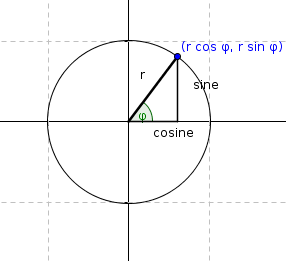
\includegraphics[scale=2]{unitcircle.png}
\caption{A picture of the unit circle, the hypotenuse r, the adjacent cosine, the opposite sine and the angle $\varphi$. It is a circle of radius r, and no longer the unit circle, if $r \neq 1$.}
\end{figure}


\textbf{Remark}.The values of $r_x, r_y$ and $r_z$ decide, how long one unit into each
direction is. To preserve affine graphical transformations all three
axes should have the same length, to represent same distance for each coordinate unit. 
The units can generally be enlarged or made smaller than \emph{unit length}, which is a length of $1$. 
By default the resulting vectors with the cosine for $x$ and sine for $y$ components have \emph{unit length}, 
if you don´t multiply the cosine and the sine in each basis vector with $r_x, r_y$ and $r_z$. The $r_n$ represent the lengths of the hypotenuses or the new radius of the circle around the origin described by the vectors. \\

\textbf{Remark} On the other side, the length of $r$ can be determined from existing basis vectors.
By pulling the square root out of the sum of the squares of the vector components.
This is also known as euclidean norm, or the root of the inner product of the vector with itself.
Like real fans of sines and cosines, we know that $\sin^2 \varphi + \cos^2 \varphi = 1$ and what the root of 1 is.
If we pull the root out of the products of cosine and sine multiplied with $r \ne 1$, we get the length of $r$ again. 
$r = \sqrt{\vec{x}\cdot\vec{x}}$ = $\sqrt{(\vec{x},\vec{x})}$ = $\left(\Sigma_{i=1}^{n} \vec{x}_i^2\right)^{\frac{1}{2}}$ = $\|\vec{x}\|$\\

\subsection{Lemma of the orthogonal bases}\\

\textbf{Remark.} Not corrected in this version, i can use the word \emph{basis} together with the formula without the adjective. New lecture scripts proved me. The orthogonal case is then taught a paragraph later.\\

The one lemma we need is the generic theorem for multiplying a vector with some basis for some coordinate system.\\

In our case the orthogonality by 90 degrees rules do not count. The basis vectors are no longer perpendicular. Or in other words
$\neg \left( \vec{e}_i \perp \vec{e}_j \right)$ with $i,j \in \{x,y,z\}.$

The plane gives us two degrees of freedom\footnote{A version later i am asking myself, if i may use degree of freedom? According to https://de.wikipedia.org/wiki/Freiheitsgrade. Maybe i have explained it understandable, but wrong now.}, to go horizontal or vertical. And in a cartesian coordinate system with infinite points, we can choose any direction around a point (x,y).
Any not straight move will go horizontally or vertically by componentwise amounts. Any straight move will go by one of the components only.
We arrange for example with about 120 degrees\footnote{The angle between $e_x$ and $e_y$ can be a little bigger, if $e_z$ points up. I have noticed this on pictures. And before you get crazy, you are allowed to choose any angles. Let x,y be perpendicular or smaller. It is your choice.} between each axis around the origin on a plane. \\

The point is, the generic formula still holds.\\
The formula for multiplying a vector with a base to get a new vector is this.\footnote{The formula can be found in many mathematics, chemistry and physics lecture scripts, and a good introduction is \cite{Strang1}.\\}

\begin{displaymath}
\vec{v} = \displaystyle\sum_{i=1}^{n} \vec{x}_i\vec{e}_i
\end{displaymath}

It is done componentwise for each row of the vector. $n$ is the number of the source dimensions. In our case it is $n = 3$. 
We are summing three products for each component of the new vector. Our old $\vec{x}$ is a $\vec{x} \in \mathbb{R}^3$.\\
With $\vec{x}_i$ as the coordinate component and $\vec{e}_i$ as the corresponding basis vector and the current component. $\vec{v}$ is the resulting new vector. 
The new vector $\vec{v}$ is a $\vec{v} \in \mathbb{R}^2$.\\

This is also equal to

\begin{displaymath}
\vec{v} = x\vec{i} + y\vec{j} + z\vec{k}
\end{displaymath}

what also explains, what the ijk-Notation means. If you don´t use it already for determining determinants for
calculating cross products. It is for describing a vector. Don´t forget, our $i, j, k$ basis is two dimensional, 
because we draw on a 2-D plane like the computer screen or a piece of paper. \\

With a 3x3 basis the vector $x\vec{i} + y\vec{j} + z\vec{k}$ is equal to \left(\begin{array}{1}x'\\y'\\z'\end{array}\right)$. But with a 2x3 basis the vector $x\vec{i} + y\vec{j} + z\vec{k}$ is becoming  \left(\begin{array}{1}x'\\y'\end{array}\right)$\\

\subsection{Finishing the matrix}\\

Each $(x,y,z)$ coordinate has to be multiplied for the new $(x',y')$
with it´s corresponding term of the basis vectors in the matrix. That means,
to sum the products with $(x,y,z)$ and the cos terms up for $x'$ and to sum the products
of $(x,y,z)$ and the sin terms up for $y'$. This is the same as imagining walking left and
right with $\cos \varphi$ and up and down with $\sin \varphi$. Or mathematically adding positive or negative values.\\

\begin{displaymath}
\left(\begin{array}{1}x'\\y'\end{array}\right) = \left(\begin{array}{1}
xr_x\cos(\varphi_x) + yr_y\cos(\varphi_y) + zr_z\cos(\varphi_z)\\
xr_x\sin(\varphi_x) + yr_y\sin(\varphi_y) + zr_z\sin(\varphi_z)\end{array}\right)\\
\end{displaymath}\\

\textbf{Remark} The sum of the basis multiplied with the coordinates is nothing
new. But literature and lecture scripts just tell how to multiply
same dimensions, giving no clue about the easy 3-D to 2-D conversions.
I can not speak for all, and do not believe, that no one told no one about this, 
but i have not met any one in the last twenty years telling me about this easy 
transformation and computer graphics went another, more complicated way, over
homogeneous coordinates, 4 by 4 matrices and a final viewport division, to get
the points back to two dimensions.\\

\section{Theorem}
\subsection{The transformation matrix}
\index{Definition}
\newtheorem{Definition}{Definition}
\begin{Definition}
Let \boldsymbol{A} be the matrix containing the three, two dimensional and trigonometric, basis vectors in order, one each
column. You get a rectangular 2x3 matrix $\boldsymbol{A} \in \mathbb{R}^{2x3}: \mathbb{R}^{3} \rightarrow \mathbb{R}^{2}$. With the basis vectors $\left(\begin{array}{1}r_n \cos \varphi_n\\r_n \sin \varphi_n\end{array}\right)$ in the three columns. 

\begin{displaymath}
\boldsymbol{A} := \begin{pmatrix}
    \vec{e}_x & \vec{e}_y & \vec{e}_z
    \end{pmatrix}
    = 
    \begin{pmatrix}
    r_x\cos(\varphi_x) & r_y\cos(\varphi_y) & r_z\cos(\varphi_z) \\
    r_x\sin(\varphi_x) & r_y\sin(\varphi_y) & r_z\sin(\varphi_z) \\
    \end{pmatrix}\\

\end{displaymath}\\

\boldsymbol{A} should be treated as a function $\boldsymbol{A} \in \mathbb{R}^{2x3} : \mathbb{R}^3 \rightarrow \mathbb{R}^2$. ($\vec{x}) \mapsto \boldsymbol{A}\vec{x}$. 
\end{Definition}\\

\subsection{The transformation}
\index{Theorem}
\newtheorem{Theorem}{Theorem (The Fundamental Theorem of transforming 3-D Points into 2-D Points)}
\begin{Theorem}\\

If you multiply \boldsymbol{A}, the matrix of the three two-dimensional basis vectors,
with the three-coordinate point $(x,y,z)$, the result is a two coordinate point, 
$(x',y')$. This point $(x',y')$ is the correct point on the two dimensional plane,
representing the point $(x,y,z)$ from the three dimensional coordinate system, you are transforming.\\

\begin{displaymath}
\boldsymbol{A}\left(\begin{array}{1}x\\y\\z\end{array}\right) = \left(\begin{array}{1}x'\\y'\end{array}\right)
\end{displaymath}

Applying the operator performs the following operation\\

\begin{equation*}
\begin{displaymath}
\boldsymbol{A}\left(\begin{array}{1}x\\y\\z\end{array}\right) = x\vec{e}_x + y\vec{e}_y + z\vec{e}_z\\
%\end{displaymath}
%\begin{displaymath}
&= \left(\begin{array}{1}xr_x\cos(\varphi_x) + yr_y\cos(\varphi_y) + zr_z\cos(\varphi_z)\\
xr_x\sin(\varphi_x) + yr_y\sin(\varphi_y) + zr_z\sin(\varphi_z)\\
\end{array}\right) = \left(\begin{array}{1}x'\\y'\end{array}\right)
\end{displaymath}
\end{equation*}

\end{Theorem}

\textbf{Proof}\\
\begin{displaymath}
\boldsymbol{A}\left(\begin{array}{1}x\\y\\z\end{array}\right) = x\vec{e}_x + y\vec{e}_y + z\vec{e}_z = \left(\begin{array}{1}x'\\y'\end{array}\right)
\end{displaymath}

\begin{displaymath}
\left(\begin{array}{1}x'\\y'\end{array}\right) = \left(\begin{array}{1}
xr_x\cos(\varphi_x) + yr_y\cos(\varphi_y) + zr_z\cos(\varphi_z)\\
xr_x\sin(\varphi_x) + yr_y\sin(\varphi_y) + zr_z\sin(\varphi_z)\end{array}\right)
\end{displaymath}\\

\subsection{Computer implementations of the matrix and the transformation}
\subsubsection{Generic computer code}
\begin{example}
The following is example code for various computer systems.\\
\begin{lstlisting}
x_ = x*r*cos(alpha) + y*r*cos(beta) + z*r*cos(gamma)
y_ = x*r*sin(alpha) + y*r*sin(beta) + z*r*sin(gamma)
\end{lstlisting}
\end{example}\\


\subsubsection{JavaScript computer code}
\begin{example}
This is a full EcmaScript 6 snippet with all neccessary informations.\\
\begin{lstlisting}
let rad = (deg) => Math.PI/180*deg;
let r_x = 1, r_y = 1, r_z = 1; 
let phi_x = rad(220), phi_y = rad(330), phi_z = rad(90); 
let xAxisCos = r_x*Math.cos(phi_x), 
    yAxisCos = r_y*Math.cos(phi_y),
    zAxisCos = r_z*Math.cos(phi_z),
    xAxisSin = r_x*Math.sin(phi_x), 
    yAxisSin = r_y*Math.sin(phi_y),
    zAxisSin = r_z*Math.sin(phi_z);
let transform2d = ([x,y,z]) => [
    x*xAxisCos+ y*yAxisCos+ z*zAxisCos,
    x*xAxisSin+ y*yAxisSin+ z*zAxisSin];
let transform2dAll = (P) => P.map(transform2d);

let examplePoints = transform2dAll([[1,2,3], [3,4,5], [14,24,15]]);
\end{lstlisting}
\end{example}\\

\textbf{Remark} I already proved affine transformations (Rotation, Scaling, Translation),
with and without applying a local 3x3 base to the object (with is better, let $r_x = r_y = r_z$), then projecting the points afterwards with 
this formula. I think the alternative graphics algorithm up to there could find a place here.\\




\begin{figure}[h]
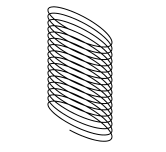
\includegraphics[scale=0.5]{helix.png}
\caption{A helix (35*Math.cos(t), 15*Math.sin(t), t) shown as (x,y,z)=f(t) with implement.html on a Canvas2DRenderingContext testing the javascript example code.}
\end{figure}



\begin{figure}[h]
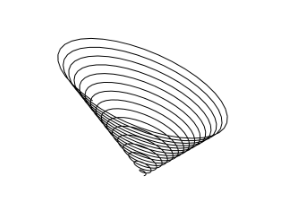
\includegraphics[scale=0.5]{conicalhelix.png}
\caption{A conical helix (t/2*Math.cos(t), t*Math.sin(t), t) shown as (x,y,z)=f(t) with implement.html on a Canvas2DRenderingContext testing the javascript example code.}
\end{figure}




\begin{figure}[h]
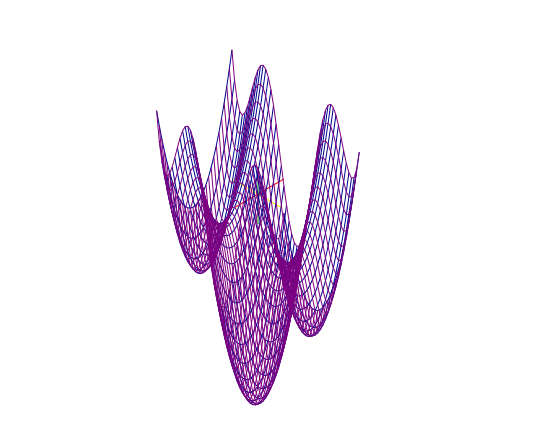
\includegraphics[scale=0.33]{fxyplot.png}
\caption{$x^2 + y^2 + 3y \sin y$  from [-5,5] and [-3,3] as z=f(x,y) with cheap3danimate.html on a Canvas2DRenderingContext}
\end{figure}



\section{Corollary}

\subsection{Converting four Dimensions down to two dimensions}\\

The theorem can be used to handle more dimensions, for example can four two-dimensional
vectors represent a 4-D space on the 2-D plane. They get converted into the correct
2-D points. For Example, if you use a 2x4 matrix and convert all points at each 
instance of $t$ you have a moving object into the direction of the fourth basis vector. \\

\begin{displaymath}
\boldsymbol{A} := \begin{pmatrix}
    \vec{e}_x & \vec{e}_y & \vec{e}_z & \vec{e}_t\end{pmatrix}\\ = 
    \begin{pmatrix}
    r_x\cos(\varphi_x) & r_y\cos(\varphi_y) & r_z\cos(\varphi_z) & r_t\cos(\varphi_t)\\
    r_x\sin(\varphi_x) & r_y\sin(\varphi_y) & r_z\sin(\varphi_z) & r_t\sin(\varphi_t)\\
    \end{pmatrix}
\end{displaymath}

Here the basis is four times of two dimensions. A 2x4 matrix with four two dimensional basis vectors, one for each axis.\\

\begin{displaymath}
\boldsymbol{A}\left(\begin{array}{1}x\\y\\z\\t\end{array}\right) = \sum_{n} \vec{e}_n\vec{x}_n = \left(\begin{array}{1}x'\\y'\end{array}\right)\\
\end{displaymath}

\textbf{Proof}:

\begin{displaymath}
\boldsymbol{A}\left(\begin{array}{1}x\\y\\z\\t\end{array}\right) &= \left(\begin{array}{1}
xr_x\cos(\varphi_x) + yr_y\cos(\varphi_y) + zr_z\cos(\varphi_z) + zr_t\cos(\varphi_t)\\
xr_x\sin(\varphi_x) + yr_y\sin(\varphi_y) + zr_z\sin(\varphi_z)+ zr_t\sin(\varphi_t)\end{array}\right)\\
\end{displaymath}
\begin{displaymath}
&= x\vec{e}_x + y\vec{e}_y + z\vec{e}_z + t\vec{e}_t &= \sum_{n} \vec{e}_n\vec{x}_n &= \left(\begin{array}{1}x'\\y'\end{array}\right)
\end{displaymath}\\

The same method can be used to convert any other number of dimensions to the $xy$-plane. But it can also be
used in a generic m by n case\footnote{http://de.wikipedia.org/wiki/Abbildungsmatrix, also found in lecture scripts, but not anyone explaining me this matrix here or the topic of the from-three-to-two-points conversion. Is it too obvious? Or isn´t it obvious?}, to convert from n dimensions down to m, if you know the basis for the destination.\\

\section{Summary}

\subsection{Summary of all neccessary steps}
\begin{enumerate}
\item Lay out the three basis vectors around a circle and write down the angles $\varphi_n$. Programmers have to write down a variable for anyways.
\item Write down the basis vectors $\vec{e}_n$ as $r_n \cos \varphi_n$ and $r_n \sin \varphi_n$ (two dimensional). Don´t multiply with $r_n$ for a unit length of $1$ or multiply with $r_n$ to change the length of the basis vector.
\item Put the three basis vectors $\vec{e}_n$ into a matrix \bigsymbol{A}. Programmers can directly code the two lines of multiplication and forget the formal rest.
\item Iterate over your points and multiply each $(x,y,z)$ with the matrix \boldsymbol{A}, which acts as a linear operator, and put $(x',y')$ into your new set.
\end{enumerate}

\textbf{Remark}\\
About the word \emph{unit}. I am not really sure, if i have to use \emph{base vector} for a vector of any length and \emph{unit vector} only for the \emph{unit length} of $1$. Because of the misleading mismatch with the \emph{unit} of the thought \emph{coordinate axes}, which the \emph{base vector} defines, i tend in the first versions to misuse the word \emph{unit vector} for both. If you find this, or any other formal mistake, be sure, it is not wanted :-) I will try to remove more of these spelling errors\footnote{The \emph{Gerholdian operator}, the \emph{Gerholdian basis}, the \emph{Gerhold projection matrix}, the \emph{Gerhold transformation} are my favourite nicknames for my late discovery, making sure, the three two dimensional and trigonometric basis vectors, which i explained, sit in the matrix.} in the next versions.


\begin{thebibliography}    

    \bibitem{Corral1} \textit{Michael Corral, Schoolcraft College},
        Vector Calculus, GNU Free Documentation License, http://mecmath.net 
        
    \bibitem{Corral2} \textit{Michael Corral, Schoolcraft College},
        Trigonometry, GNU Free Documentation License, http://mecmath.net         
        
    \bibitem{Strang1} \textit{Gilbert Strang, MIT},
        Linear Algebra and it´s Applications. Fourth Edition.
        
    \bibitem{Strang2} \textit{Gilbert Strang, MIT},
            Calculus. MIT OpenCourseWare Supplemental Resources. http://ocw.mit.edu    
            
    \bibitem{Corral3} \textit{Michael Corral, Schoolcraft College},
            Latex Mini Tutorial, http://mecmath.net            
            
    \bibitem{Jürgens,Feuerstack} \textit{Manuela J\"urgens, Thomas Feuerstack, Fernuniversit\"at Hagen},
            LaTeX, eine Einf\"uhrung und ein bisschen mehr..., a026\_latex\_einf.pdf
            
    \bibitem{Rudl} \textit{Dr.Jan Rudl, Technische Universit\"at Dresden, Fachbereich Mathematik},
            Einf\"uhrung in LaTeX, LaTeX-Kurs.pdf            

\end{thebibliography}



\appendix

\section{Proving more rules of vector spaces}\\

\subsection{The origin stays in the origin}

A trivial proof is to prove, that the zero vector $\vec{0} \in \mathbb{R}^3$ maps to the zero vector $\vec{0} \in \mathbb{R}^2$.\\

\textbf{Proof}:
\begin{displaymath}
    \boldsymbol{A}\left(\begin{array}{1}0\\0\\0\end{array}\right)
    = \left(\begin{array}{1}0 + 0 + 0\\0 + 0 + 0\end{array}\right) 
    =\left(\begin{array}{1}0\\0\end{array}\right)
\end{displaymath}\\

\subsection{Points along one axis}

Another trivial proof is to prove, that coordinates lying on one axis are a multiple of the basis vector of the axis.\\

\textbf{Proof}:
\begin{displaymath}
    \boldsymbol{A}\left(\begin{array}{1}a\\0\\0\end{array}\right)
    = \left(\begin{array}{1}ar_x\cos \varphi_x + 0 + 0\\ar_x\sin \varphi_x  + 0 + 0\end{array}\right) 
    = a\vec{e}_x
\end{displaymath}

\begin{displaymath}
    \boldsymbol{A}\left(\begin{array}{1}0\\1\\0\end{array}\right)
    = \left(\begin{array}{1}0 + r_y\cos \varphi_y + 0\\0 + r_y\sin \varphi_y + 0\end{array}\right) 
    = \vec{e}_y
\end{displaymath}

\begin{displaymath}
    \boldsymbol{A}\left(\begin{array}{1}0\\0\\-b\end{array}\right)
    = \left(\begin{array}{1}0 + 0 - br_z\cos \varphi_z\\0 + 0 - br_z\sin \varphi_z\end{array}\right) 
    = -b\vec{e}_z
\end{displaymath}\\

\subsection{Multiplications with constants}

Another trivial proof is to show, that $\boldsymbol{A}(\lambda\vec{x}) = \lambda\boldsymbol{A}\vec{x}$. It doesn´t matter, where you multiply with the constant. You can multiply the original vector, or the resulting vector. You reach the same point.\\

\textbf{Proof}:\\
\begin{displaymath}
\begin{equation*}
\begin{align*}
\boldsymbol{A}(\lambda\vec{x}) &= \boldsymbol{A}\left(\begin{array}{1}\lambda{x}\\\lambda{y}\\\lambda{z}\end{array}\right)\\ &= \left(\begin{array}{1}\lambda{x}r_x\cos(\varphi_x) + \lambda{y}r_y\cos(\varphi_y) + \lambda{z}r_z\cos(\varphi_z)\\
\lambda{x}r_x\sin(\varphi_x) + \lambda{y}r_y\sin(\varphi_y) + \lambda{z}r_z\sin(\varphi_z)
\end{array}\right)\\
    &= \lambda\left(\begin{array}{1}xr_x\cos(\varphi_x) + yr_y\cos(\varphi_y) + zr_z\cos(\varphi_z)\\
xr_x\sin(\varphi_x) + yr_y\sin(\varphi_y) + zr_z\sin(\varphi_z)\\
\end{array}\right)\\
    &= \lambda\left(\begin{array}{1}x'\\y'\end{array}\right)\\
    &= \lambda\boldsymbol{A}\vec{x}
\end{align*}
\end{equation*}
\end{displaymath}\\


\subsection{Additions and subtractions}

Another trivial proof is to show, that $\boldsymbol{A}(\vec{v} + \vec{w}) = \boldsymbol{A}\vec{v} + \boldsymbol{A}\vec{w}$. 
It does not matter, if you add the original or the results . The outcome is the same point, the same vector.\\
 
\textbf{Proof}:\\

\begin{displaymath}
\begin{equation*}
\begin{align*}
\boldsymbol{A}\left(\begin{array}{1}x+u\\y+v\\z+w\end{array}\right) &= \left(\begin{array}{1}(x+u)r_x\cos(\varphi_x) + (y+v)r_y\cos(\varphi_y) + (z+w)r_z\cos(\varphi_z)\\
(x+u)r_x\sin(\varphi_x) + (y+v)r_y\sin(\varphi_y) + (z+w)r_z\sin(\varphi_z)\\
\end{array}\right)\\
            &= \left(\begin{array}{1}xr_x\cos(\varphi_x) + yr_y\cos(\varphi_y) + zr_z\cos(\varphi_z)\\
xr_x\sin(\varphi_x) + yr_y\sin(\varphi_y) + zr_z\sin(\varphi_z)\\
\end{array}\right) + \left(\begin{array}{1}ur_x\cos(\varphi_x) + vr_y\cos(\varphi_y) + wr_z\cos(\varphi_z)\\
ur_x\sin(\varphi_x) + vr_y\sin(\varphi_y) + wr_z\sin(\varphi_z)\\
\end{array}\right)\\    
    &= \left(\begin{array}{1}x'\\y'\end{array}\right) + \left(\begin{array}{1}u'\\v'\end{array}\right)\\
    &= \boldsymbol{A}\left(\begin{array}{1}x\\y\\z\end{array}\right) + \boldsymbol{A}\left(\begin{array}{1}u\\v\\w\end{array}\right)
\end{align*}
\end{equation*}
\end{displaymath}
\subsection{Rule of linearity}

\textbf{Corollary} From the previous two proofs, it is obvious to see, that
\begin{displaymath}
\boldsymbol{A}(\lambda\vec{v} + \kappa\vec{w}) = \lambda\boldsymbol{A}\vec{v} + \kappa\boldsymbol{A}\vec{w} = \lambda\left(\begin{array}{1}x'\\y'\end{array}\right) + \kappa\left(\begin{array}{1}u'\\v'\end{array}\right)\\
\end{displaymath}
which is a standard formulation of the rule of linearity. For example, you can find this rule in the form $\boldsymbol{A}(c\vec{x} + d\vec{y}) = c\boldsymbol{A}\vec{x} + d\boldsymbol{A}\vec{y}$ in \cite{Strang1}, but also in every linear algebra 1 lecture script.\\


\subsection{About the norm}

The norm used is the euclidean norm, or the 2-norm. This is the square root of the sum of the squares of the absolute values of the components $\|\vec{x}\| = \sqrt{\sum_{i=1}^{n}|x_n|^2}$. In linear algebra, functional analysis and topology lectures there are three fundamental properties of the norm. Definiteness, homogenity and the triangle inequality.\\


\textbf{Definitness} Show that $\|\vec{x}\| = 0$ if $\vec{x} = 0$\\
\begin{displaymath}
    \|\vec{x}\| = \|\vec{0}\| = \sqrt{0^{2} + 0^{2}} = 0
\end{displaymath}\\

\textbf{Homogenity} Show that $\|a\vec{x}\| = |a|\|\vec{x}\|$\\
\begin{displaymath}
    \|a\vec{x}\| = \sqrt{|a\vec{x}_1|^{2} + |a\vec{x}_2|^{2}} = \sqrt{|a|^{2}(|\vec{x}_1|^{2} + |\vec{x}_2|^{2})} = |a|\sqrt{|\vec{x}_1|^{2} + |\vec{x}_2|^{2}} = |a|\|\vec{x}\|
\end{displaymath}\\

\textbf{Triangle inequality} (Minkowski inequality) Show that $ \|\boldsymbol{A}(\vec{v} + \vec{w})\| \leq \|\boldsymbol{A}\vec{v}\| + \|\boldsymbol{A}\vec{w}\|$\\

\begin{displaymath}
    \sqrt{\sum_{i=1}^{n}|\vec{v}_i + \vec{w}_i|^{2}} \leq \sqrt{\sum_{i=1}^{n}|\vec{v}_i|^{2}} + \sqrt{\sum_{i=1}^{n}|\vec{w}_i|^{2}} 
\end{displaymath}\\

\textbf{Remark} This subsection is not complete.

\subsection{Metrics}

Where a norm is, there will be a metric induced.
The measurement of the distance between two points is defined by the d-function. It is the length of the difference vector between the two points.\\
\begin{displaymath}
    d(\vec{x}, \vec{y}) = \|\vec{x}-\vec{y}\| = \sqrt{\sum_{i=1}^{n}|\vec{x}_i-\vec{y}_i|^2}
\end{displaymath}

Metrics have three fundamental properties.
\begin{enumerate}
\item If the distance is zero, the vectors are equal.
\begin{displaymath}
d(x,y) = 0 \iff x = y
\end{displaymath}
\item It does not matter, whether you read $d(x,y)$ or $d(y,x)$, the number must be equal.
\begin{displaymath}
d(x,y) = d(y,x)
\end{displaymath}
\item The third one is the triangle inequality. Going over another point is always a step longer.
\begin{displaymath}
d(x,z) \leq d(x,y) + d(y,z) 
\end{displaymath}
\end{enumerate}


\textbf{Remark} This subsection is not complete and has to be continued. The point is to measure now the difference between the original coordinates and the new planar coordinates. $d(\vec{x}, \vec{y})_2 = \|\vec{x}-\vec{y}\|_2 \leq d(\vec{x}, \vec{y})_3 = \|\vec{x}-\vec{y}\|_3$ is my assumption which is not proven now.

\subsection{Transpose and unproven}

\textbf{Remark} Less trivial is to figure out, what the transpose and the products with the transpose and the inverse matrices of those products are good for. Our rectangular 2x3 basis matrix has a transponse. A 3x2 matrix. The products are $\boldsymbol{A}\boldsymbol{A}^T$, a 2 by 2 matrix, and $\boldsymbol{A}^T\boldsymbol{A}$, a 3 by 3 matrix. Today i will just show the transpose. \\

\begin{displaymath}
\left(
    \begin{array}{111}
    r_x\cos(\varphi_x) & r_y\cos(\varphi_y) & r_z\cos(\varphi_z) \\
    r_x\sin(\varphi_x) & r_y\sin(\varphi_y) & r_z\sin(\varphi_z) \\
    \end{array}
\right)^T
= \left(
    \begin{array}{11}
    r_x\cos(\varphi_x) & r_x\sin(\varphi_x)\\
    r_y\cos(\varphi_y) & r_y\sin(\varphi_y)\\
    r_z\cos(\varphi_z) & r_z\sin(\varphi_z) \\
    \end{array}
\right)
\end{displaymath}\\

Multiplying out the transposes yield the following forms.

\begin{displaymath}
\boldsymbol{A}\boldsymbol{A}^T = \begin{pmatrix} 
\sum_{i=1}^{3}r_n\cos\varphi_n & \sum_{i=1}^{3}r_n^2\cos\varphi_n\sin\varphi_n\\
\sum_{i=1}^{3}r_n^2\cos\varphi_n\sin\varphi_n & \sum_{i=1}^{3}r_n\sin\varphi_n
\end{pmatrix} = \begin{pmatrix}a & b\\b & c
\end{pmatrix}

You see, in the 2x2 matrix $\boldsymbol{A}\boldsymbol{A}^T$ is $a_{ij} = a_{ji}$. In the 3x3 matrix $\boldsymbol{A}^T\boldsymbol{A}$ is also $a_{ij} = a_{ji}$. I will abbreviate $\cos \varphi_n$ with $C_n$ and
$\sin \varphi_n$ with $S_n$.

\textbf{Remark} I have not compared with the sin(A+B) formulas.

\begin{displaymath}
\boldsymbol{A}^T\boldsymbol{A} = \begin{pmatrix} 
    C_x^2+S_x^2 & C_xC_y+S_xS_y & C_xC_z+S_xS_z\\
    C_yC_x+S_yS_x & C_y^2+S_y^2 & C_yC_z+S_yS_z\\
    C_zC_x+S_zS_x & C_zC_y+S_zS_y & C_z^2+S_z^2
\end{pmatrix}
= \begin{pmatrix}
    r_x^2 & a & b \\
    a & r_y^2 & c \\
    b & c & r_z^2 \\
\end{pmatrix}
\end{displaymath}

\textbf{Remark} I wrote down the formula for the 2x2 determinant and noticed, it´s getting hairy writing with bare hands. Using numeric software like FreeMat should be less stressing. Whether it makes sense to calculate the determinants and the inverses or
not, can not be told from looking at these matrices by a guy like me. This topic is continued in the next versions.

\textbf{Remark} Missing are $|\boldsymbol{A}\boldsymbol{A}^T|$ and $|\boldsymbol{A}^T\boldsymbol{A}|$ and $(\boldsymbol{A}\boldsymbol{A}^T)^{-1}$ and $(\boldsymbol{A}^T\boldsymbol{A})^{-1}$ and various tries to combine them to $P$, to $x^TAx$, and and.



\section{An alternative graphics algorithm}

\textbf{Remark} This section is new on July 10.

With the new information how to translate the coordinates, it is obvious, that we want to draw some graphics on our 2-D Canvas.
By doing so, i already found out a few interesting points of how to do this. Without homogenous coordinates or 4 by 4 matrices.\\

\subsection{Origin}  

Setting the origin is an easy task. Assuming, the regular origin is at (0,0,0) and (0,0), we just need to add the shift to the coordinate. You can shift the 3-D Origin or the 2-D Origin.\\
\begin{lstlisting}
x = Ox + x;
y = Oy + y;
z = Oz + z;
\end{lstlisting}

\subsection{Translation}

Translating the points is very easy without a 4 by 4 matrix. You simply add the translation vector to each point.\\

\begin{lstlisting}
x = Tx + x;
y = Ty + y;
z = Tz + z;
\end{lstlisting}

\subsection{Scaling}

To scale the object you just have to multiply with the constant. Reflecting, that it is no difference, whether you multiply
before or after the transformation, you can choose, what to scale, the 3-D or the 2-D object.\\

\begin{lstlisting}
x = Sx * x;
y = Sy * y;
z = Sz * z;
\end{lstlisting}

\subsection{Local 3x3 basis}

If you wish to introduce different units into different directions, you have to apply a local basis. Applying the local 3x3
basis to an object makes it rotatable with changed units. If you change the units of r on the projection, rotation may give unrealistic results since suddenly the object stretches to an unexpected size. \\

The matrix applied locally is a 3x3 matrix $\begin{pmatrix} xBX & yBX & zBX\\ xBY & yBY & zBY\\ xBZ & yBZ & zBZ\end{pmatrix}$.
For example is $\begin{pmatrix} 1 & 0 & 0\\ 0 & 1 & 0\\ 0 & 0 & 1\end{pmatrix}$ is an orthogonal standard basis and the result is the same as if you do not apply any basis to the object, as the assumed default coordinate system in $R^{3}$ is orthogonal.

\begin{lstlisting}
u = x, v = y, w = z;
x = u*xBX + v*yBX + w*zBX;
y = u*xBY + v*yBY + w*zBY;
z = u*xBZ + v*yBZ + w*zBZ;
\end{lstlisting}

This of course transform the object by the directions and the length of the three three dimensional basis vectors.


\subsection{Rotation}

Rotating the object can be done in three dimensional space by applying the regular rotation matrices

\begin{lstlisting}
    u = x, v = y, w = z;
    y = v * rotxcos - w * rotxsin
    z = v * rotxsin + w * rotxcos
    u = x, v = y, w = z;
    x = u * rotycos + w * rotysin;
    z = -u * rotysin + w * rotycos;
    u = x, v = y, w = z;
    x = u * rotzcos - v * rotzsin;
    y = u * rotzsin + v * rotzcos;
\end{lstlisting}

\textbf{Remark} I have to remove the substitution and write the whole thing out again. Next version.

\subsection{Code Example}

Last but not least here is a code snippet doing all the things together, showing you the order of transformation.


\printindex
\end{document}